% ICCV 2025 Paper Template; see https://github.com/cvpr-org/author-kit

\documentclass[10pt,twocolumn,letterpaper]{article}

%%%%%%%%% PAPER TYPE  - PLEASE UPDATE FOR FINAL VERSION
%\usepackage{iccv}              % To produce the CAMERA-READY version
%\usepackage[review]{iccv}      % To produce the REVIEW version
\usepackage[pagenumbers]{iccv} % To force page numbers, e.g. for an arXiv version

% Import additional packages in the preamble file, before hyperref
\usepackage[dvipsnames]{xcolor}
\definecolor{thedarkblue}{RGB}{0,0,120} %
\definecolor{mydarkblue}{rgb}{0,0.08,0.45} %
\definecolor{darkblue}{rgb}{0,0.08,180}
\colorlet{TufteRed}{red!80!black}
\definecolor{theblue}{RGB}{0,0,180}
\colorlet{thered}{TufteRed}
      
\usepackage{microtype}
\usepackage{balance}


\usepackage{booktabs}
\usepackage{tabularx}



\renewcommand{\qedsymbol}{$\blacksquare$}
\newcommand{\eat}[1]{\ignorespaces}
\usepackage{comment}

\usepackage{tikz}
\usepackage{verbatim}
\usetikzlibrary{arrows}
\usetikzlibrary{shapes,snakes}
\usetikzlibrary{decorations.pathmorphing} %
\usetikzlibrary{fit}					%
\usetikzlibrary{backgrounds}	%

\usepackage{ragged2e}
\usepackage{makecell}
\usepackage{multirow}
\usepackage{microtype}
\usepackage{balance}
\usepackage{setspace}

\graphicspath{{./}{./graphics/}}
\newcolumntype{H}{>{\setbox0=\hbox\bgroup}c<{\egroup}@{}}

\newcolumntype{R}[1]{>{\RaggedLeft\arraybackslash}} %
\newcolumntype{L}[1]{>{\RaggedRight\arraybackslash}} %

\newcommand\TTT{\rule{0pt}{3.2ex}}
\newcommand\BBB{\rule[-1.4ex]{0pt}{0pt}}


\newcommand{\rbr}[1]{\left(#1\right)}
\newcommand{\cbr}[1]{\left\{#1\right\}}
\newcommand{\nbr}[1]{\left\|#1\right\|}
\newcommand{\abr}[1]{\left|#1\right|}
\newcommand{\abs}[1]{\left|#1\right|}
\newcommand{\floor}[1]{\left\lfloor #1 \right\rfloor}
\newcommand{\ceil}[1]{\left\lceil #1 \right\rceil}
\newcommand{\inner}[2]{\left\langle #1,#2 \right\rangle}

\newcommand{\etal}{\emph{et al.}}
\newcommand{\ea}{\emph{et al.}}
\newcommand{\eg}{\emph{e.g.}}
\newcommand{\ie}{\emph{i.e.}}
\newcommand{\iid}{\emph{iid}}
\newcommand{\cf}{\emph{cf.}\ }
\newcommand{\wrt}{\emph{w.r.t.}\ }
\newcommand{\st}{\emph{s.t.}\ }

\newtheorem{corollary}{\bfseries{Corollary}}
\newtheorem{proof2}{PROOF}
\newtheorem*{fact}{Fact}
\newtheorem*{note}{\hspace{-1em}\textsc{Note}}
\newtheorem{corol}{Corollary}%
\newtheorem{axiom}{Axiom}%
\newtheorem{cond}{Condition}%
\newtheorem{property2}{Property}%
\newtheorem{property}{Property}%
\newtheorem{lemma}{\hspace{-1em}\bfseries{Lemma}}
\newtheorem{Definition}{\hspace{-1em}\bfseries{Definition}}
\newtheorem{Claim}{Claim}%

\AtBeginEnvironment{pmatrix}{\setlength{\arraycolsep}{2pt}}



\providecommand{\tensor}[1]{\boldsymbol{\mathcal{#1}}}%
\providecommand{\mat}[1]{\boldsymbol{\mathrm{#1}}}%
\renewcommand{\vec}[1]{\boldsymbol{\mathrm{#1}}}
\providecommand{\sca}[1]{{\mathrm{#1}}}%
\DeclareMathOperator{\rank}{rank}%
\DeclareMathOperator{\diag}{diag}%
\DeclareMathOperator{\Diag}{Diag}%
\providecommand{\itr}[2]{#1^{(#2)}}
\providecommand{\itn}[1]{^{(#1)}}%
\providecommand{\eps}{\varepsilon}%
\providecommand{\kron}{\otimes}
\DeclareMathOperator{\tvec}{vec}
\providecommand{\pmat}[1]{\begin{pmatrix} #1 \end{pmatrix}}
\providecommand{\bmat}[1]{\begin{bmatrix} #1 \end{bmatrix}}
\providecommand{\spmat}[1]{\left(\begin{smallmatrix} #1 \end{smallmatrix}\right)}
\providecommand{\sbmat}[1]{\left[\begin{smallmatrix} #1 \end{smallmatrix}\right]}

\DeclareMathOperator*{\minimize}{minimize}
\DeclareMathOperator*{\maximize}{maximize}
\DeclareMathOperator*{\argmax}{argmax}
\DeclareMathOperator*{\argmin}{argmin}
\DeclareMathOperator*{\argsort}{arg\,sort}
\providecommand{\subjectto}{\ensuremath{\text{subject to}}}
\providecommand{\MINof}[1][]{{\displaystyle \minimize_{#1}}}
\providecommand{\MIN}[2]{\begin{array}{ll} \MINof[#1] & #2 \end{array}}
\providecommand{\MINone}[3]{\begin{array}{ll} \MINof[#1] & #2 \\ \subjectto  & #3 \end{array}}
\providecommand{\MINtwo}[4]{\begin{array}{ll} \MINof[#1] & #2 \\ \subjectto  & #3 \\ & #4 \end{array}}
\providecommand{\MINthree}[5]{\begin{array}{ll} \MINof[#1] & #2 \\ \subjectto  & #3 \\ & #4 \\ & #5 \end{array}}
\providecommand{\MINfour}[6]{\begin{array}{ll} \MINof[#1] & #2 \\ \subjectto  & #3 \\ & #4 \\ & #5 \\ & #6 \end{array}}
\providecommand{\MAXof}[1][]{{\displaystyle \maximize_{#1}}}
\providecommand{\MAX}[2]{\begin{array}{ll} \MAXof[#1] & #2 \end{array}}
\providecommand{\MAXone}[3]{\begin{array}{ll} \MAXof[#1] & #2 \\ \subjectto & #3 \end{array}}
\providecommand{\MAXtwo}[4]{\begin{array}{ll} \MAXof[#1] & #2 \\ \subjectto  & #3 \\ & #4 \end{array}}
\providecommand{\MAXthree}[5]{\begin{array}{ll} \MAXof[#1] & #2 \\ \subjectto  & #3 \\ & #4 \\ & #5 \end{array}}
\providecommand{\MAXfour}[6]{\begin{array}{ll} \MAXof[#1] & #2 \\ \subjectto  & #3 \\ & #4 \\ & #5 \\ & #6 \end{array}}

\DeclareMathOperator{\E}{E}
\DeclareMathOperator{\hugeE}{\mbox{\huge\raise-0.3ex\hbox{E}}}
\DeclareMathOperator{\p}{\mathbb{P}}
\DeclareMathOperator{\hugep}{\mbox{\huge\raise-0.3ex\hbox{$\p$}}}
\DeclareMathOperator{\Var}{Var}
\DeclareMathOperator{\Cov}{Cov}
\DeclareMathOperator{\Bias}{Bias}
\DeclareMathOperator{\sign}{sign}
\DeclareMathOperator{\Std}{Std}
\providecommand{\Eof}{\E\BracketOf}
\providecommand{\hugeEof}{\hugeE\BracketOf}
\providecommand{\Stdof}{\Std\BracketOf}
\providecommand{\varof}{\Std\BracketOf}
\providecommand{\Covof}[2]{\Cov\BrackeOf#1,#2\right]}
\providecommand{\prob}[1][]{\p_{#1}\BraceOf}
\providecommand{\hugeprob}[1][]{\hugep_{#1}\BraceOf}

\DeclareMathOperator{\degree}{degree}
\DeclareMathOperator{\trace}{trace}
\providecommand{\set}{\mathcal}
\providecommand{\graph}{\mathcal}
\providecommand{\mathdef}{\equiv}
\providecommand{\card}{\absof}
\providecommand{\cardof}{\absof}
\providecommand{\eqdef}{\equiv}
\providecommand{\eps}{\varepsilon}
\DeclareMathOperator{\bigO}{O}
\providecommand{\bigOof}{\bigO\ParensOf}
\providecommand{\absof}[1]{$\left| #1 \right|$}

\newcommand{\RR}{\mathbb{R}}
\newcommand{\CC}{\mathbb{C}}



\providecommand{\eye}{\mat{I}}
\providecommand{\mA}{\ensuremath{\mat{A}}}
\providecommand{\mB}{\ensuremath{\mat{B}}}
\providecommand{\mC}{\ensuremath{\mat{C}}}
\providecommand{\mD}{\ensuremath{\mat{D}}}
\providecommand{\mE}{\ensuremath{\mat{E}}}
\providecommand{\mF}{\ensuremath{\mat{F}}}
\providecommand{\mG}{\ensuremath{\mat{G}}}
\providecommand{\mH}{\ensuremath{\mat{H}}}
\providecommand{\mI}{\ensuremath{\mat{I}}}
\providecommand{\mJ}{\ensuremath{\mat{J}}}
\providecommand{\mK}{\ensuremath{\mat{K}}}
\providecommand{\mL}{\ensuremath{\mat{L}}}
\providecommand{\mM}{\ensuremath{\mat{M}}}
\providecommand{\mN}{\ensuremath{\mat{N}}}
\providecommand{\mO}{\ensuremath{\mat{O}}}
\providecommand{\mP}{\ensuremath{\mat{P}}}
\providecommand{\mQ}{\ensuremath{\mat{Q}}}
\providecommand{\mR}{\ensuremath{\mat{R}}}
\providecommand{\mS}{\ensuremath{\mat{S}}}
\providecommand{\mT}{\ensuremath{\mat{T}}}
\providecommand{\mU}{\ensuremath{\mat{U}}}
\providecommand{\mV}{\ensuremath{\mat{V}}}
\providecommand{\mW}{\ensuremath{\mat{W}}}
\providecommand{\mX}{\ensuremath{\mat{X}}}
\providecommand{\mY}{\ensuremath{\mat{Y}}}
\providecommand{\mZ}{\ensuremath{\mat{Z}}}
\providecommand{\mLambda}{\ensuremath{\mat{\Lambda}}}
\providecommand{\mzero}{\ensuremath{\mat{0}}}

\providecommand{\tA}{\ensuremath{\tensor{A}}}
\providecommand{\tB}{\ensuremath{\tensor{B}}}
\providecommand{\tC}{\ensuremath{\tensor{C}}}
\providecommand{\tD}{\ensuremath{\tensor{D}}}
\providecommand{\tE}{\ensuremath{\tensor{E}}}
\providecommand{\tF}{\ensuremath{\tensor{F}}}
\providecommand{\tG}{\ensuremath{\tensor{G}}}
\providecommand{\tH}{\ensuremath{\tensor{H}}}
\providecommand{\tI}{\ensuremath{\tensor{I}}}
\providecommand{\tJ}{\ensuremath{\tensor{J}}}
\providecommand{\tK}{\ensuremath{\tensor{K}}}
\providecommand{\tL}{\ensuremath{\tensor{L}}}
\providecommand{\tM}{\ensuremath{\tensor{M}}}
\providecommand{\tN}{\ensuremath{\tensor{N}}}
\providecommand{\tO}{\ensuremath{\tensor{O}}}
\providecommand{\tP}{\ensuremath{\tensor{P}}}
\providecommand{\tQ}{\ensuremath{\tensor{Q}}}
\providecommand{\tR}{\ensuremath{\tensor{R}}}
\providecommand{\tS}{\ensuremath{\tensor{S}}}
\providecommand{\tT}{\ensuremath{\tensor{T}}}
\providecommand{\tU}{\ensuremath{\tensor{U}}}
\providecommand{\tV}{\ensuremath{\tensor{V}}}
\providecommand{\tW}{\ensuremath{\tensor{W}}}
\providecommand{\tX}{\ensuremath{\tensor{X}}}
\providecommand{\tY}{\ensuremath{\tensor{Y}}}
\providecommand{\tZ}{\ensuremath{\tensor{Z}}}

\providecommand{\ones}{\vec{e}}
\providecommand{\va}{\ensuremath{\vec{a}}}
\providecommand{\vb}{\ensuremath{\vec{b}}}
\providecommand{\vc}{\ensuremath{\vec{c}}}
\providecommand{\vd}{\ensuremath{\vec{d}}}
\providecommand{\ve}{\ensuremath{\vec{e}}}
\providecommand{\vf}{\ensuremath{\vec{f}}}
\providecommand{\vg}{\ensuremath{\vec{g}}}
\providecommand{\vh}{\ensuremath{\vec{h}}}
\providecommand{\vi}{\ensuremath{\vec{i}}}
\providecommand{\vj}{\ensuremath{\vec{j}}}
\providecommand{\vk}{\ensuremath{\vec{k}}}
\providecommand{\vl}{\ensuremath{\vec{l}}}
\providecommand{\vm}{\ensuremath{\vec{l}}}
\providecommand{\vn}{\ensuremath{\vec{n}}}
\providecommand{\vo}{\ensuremath{\vec{o}}}
\providecommand{\vp}{\ensuremath{\vec{p}}}
\providecommand{\vq}{\ensuremath{\vec{q}}}
\providecommand{\vr}{\ensuremath{\vec{r}}}
\providecommand{\vs}{\ensuremath{\vec{s}}}
\providecommand{\vt}{\ensuremath{\vec{t}}}
\providecommand{\vu}{\ensuremath{\vec{u}}}
\providecommand{\vv}{\ensuremath{\vec{v}}}
\renewcommand{\vv}{\ensuremath{\vec{v}}}
\providecommand{\vw}{\ensuremath{\vec{w}}}
\providecommand{\vx}{\ensuremath{\vec{x}}}
\providecommand{\vy}{\ensuremath{\vec{y}}}
\providecommand{\vz}{\ensuremath{\vec{z}}}
\providecommand{\vpi}{\ensuremath{\vecalt{\pi}}} 

\providecommand{\ssa}{\ensuremath{\sca{a}}}
\providecommand{\ssb}{\ensuremath{\sca{b}}}
\providecommand{\ssc}{\ensuremath{\sca{c}}}
\providecommand{\ssd}{\ensuremath{\sca{d}}}
\providecommand{\sse}{\ensuremath{\sca{e}}}
\providecommand{\ssf}{\ensuremath{\sca{f}}}
\providecommand{\ssg}{\ensuremath{\sca{g}}}
\providecommand{\ssh}{\ensuremath{\sca{h}}}
\providecommand{\ssi}{\ensuremath{\sca{i}}}
\providecommand{\ssj}{\ensuremath{\sca{j}}}
\providecommand{\ssk}{\ensuremath{\sca{k}}}
\providecommand{\ssl}{\ensuremath{\sca{l}}}
\providecommand{\ssm}{\ensuremath{\sca{l}}}
\providecommand{\ssn}{\ensuremath{\sca{n}}}
\providecommand{\sso}{\ensuremath{\sca{o}}}
\providecommand{\ssp}{\ensuremath{\sca{p}}}
\providecommand{\ssq}{\ensuremath{\sca{q}}}
\providecommand{\ssr}{\ensuremath{\sca{r}}}
\providecommand{\sss}{\ensuremath{\sca{s}}}
\providecommand{\sst}{\ensuremath{\sca{t}}}
\providecommand{\ssu}{\ensuremath{\sca{u}}}
\providecommand{\ssv}{\ensuremath{\sca{v}}}
\providecommand{\ssw}{\ensuremath{\sca{w}}}
\providecommand{\ssx}{\ensuremath{\sca{x}}}
\providecommand{\ssy}{\ensuremath{\sca{y}}}
\providecommand{\ssz}{\ensuremath{\sca{z}}}
\providecommand{\sspi}{\ensuremath{\scaalt{\pi}}} 


\DeclareMathOperator{\cut}{cut}
\DeclareMathOperator{\vol}{vol}



\definecolor{googleblue}{HTML}{4285F4}
\definecolor{googlered}{HTML}{DB4437}
\definecolor{googlepurple}{HTML}{A142F4} %
\definecolor{googlegreen}{HTML}{0F9D58}


% It is strongly recommended to use hyperref, especially for the review version.
% hyperref with option pagebackref eases the reviewers' job.
% Please disable hyperref *only* if you encounter grave issues, 
% e.g. with the file validation for the camera-ready version.
%
% If you comment hyperref and then uncomment it, you should delete *.aux before re-running LaTeX.
% (Or just hit 'q' on the first LaTeX run, let it finish, and you should be clear).
\definecolor{iccvblue}{rgb}{0.21,0.49,0.74}
\usepackage[pagebackref,breaklinks,colorlinks,allcolors=iccvblue]{hyperref}

%%%%%%%%% TITLE - PLEASE UPDATE
\title{ID-Consistent, Precise Expression Generation with Blendshape-Guided Diffusion}

%%%%%%%%% AUTHORS - PLEASE UPDATE
\author{Foivos Paraperas Papantoniou
\quad \quad \quad
Stefanos Zafeiriou\\[6pt]
Imperial College London, UK
\\{\tt\small \{f.paraperas, s.zafeiriou\}@imperial.ac.uk}
}

\begin{document}
\maketitle

\begin{strip}
\centering
\includegraphics[width=\textwidth]{figures/teaser_compressed.pdf}
\captionof{figure}{We introduce a fine-grained expression adapter on a foundation ID-consistent face model, which significantly outperforms existing approaches in expression-transfer fidelity and can apply any type of facial expression to any given subject - including extreme or asymmetric ones - using explicit blendshape parameters (left). Our method can optionally integrate a reference adapter that enables expression editing without altering the appearance or background (right).}
\label{fig:teaser}
\end{strip}

\begin{abstract}
Composed Image Retrieval (CIR), which aims to find a target image from a reference image and a modification text, presents the core challenge of performing unified reasoning across visual and semantic modalities. While current approaches based on Vision-Language Models (VLMs, e.g., CLIP) and more recent Multimodal Large Language Models (MLLMs, e.g., Qwen-VL) have shown progress, they predominantly function as ``black boxes." This inherent opacity not only prevents users from understanding the retrieval rationale but also restricts the models' ability to follow complex, fine-grained instructions. To overcome these limitations, we introduce CIR-CoT, the first end-to-end retrieval-oriented MLLM designed to integrate explicit Chain-of-Thought (CoT) reasoning. By compelling the model to first generate an interpretable reasoning chain, CIR-CoT enhances its ability to capture crucial cross-modal interactions, leading to more accurate retrieval while making its decision process transparent. Since existing datasets like FashionIQ and CIRR lack the necessary reasoning data, a key contribution of our work is the creation of structured CoT annotations using a three-stage process involving a caption, reasoning, and conclusion. Our model is then fine-tuned to produce this structured output before encoding its final retrieval intent into a dedicated embedding. Comprehensive experiments show that CIR-CoT achieves highly competitive performance on in-domain datasets (FashionIQ, CIRR) and demonstrates remarkable generalization on the out-of-domain CIRCO dataset, establishing a new path toward more effective and trustworthy retrieval systems.
\end{abstract}    
\section{Introduction}

Recently, agent systems based on Large Language Models (LLMs) have attracted significant research interest. With the rapid development of AI technologies, LLM-based agent systems dynamically handle complex tasks in various interactive environments, alleviating human burdens. Agent systems are increasingly applied across diverse fields~\citep{liu2025advances}, including clinical treatment~\citep{wang2025surveyllmbasedagentsmedicine}, scientific simulations~\citep{park2023generativeagentsinteractivesimulacra}, and software engineering~\citep{wang2025openhandsopenplatformai}.

Despite the considerable attention agent systems have received, their security remains an urgent area for improvement~\citep{wang2025comprehensivesurvey,yu2025asurveytrustagent}. One security topic previously discussed in cybersecurity yet still crucial in agent systems, is \textbf{access control (AC)}. To minimize the loss caused by privilege escalation or unexpected behavior, systems require optimal permission allocation strategies that are adapted to the generative behavior patterns of LLM-based agents. Traditional AC models, built on static rules and binary allow/deny logic~\citep{ferraiolo2009rolebasedaccesscontrols,8594462}. Early research proposed formal methods based on Information Flow Control (IFC)~\citep{myers1997decentralized} to allocate permissions, ensuring secure interactions among system entities. Subsequent advances extended these mechanisms to incorporate contextual factors such as user role, location, and time
~\citep{covington2001context}. Unfortunately, traditional IFC mechanisms face severe limitations in handling dynamic, implicit semantics or complex interactive behaviors, which renders agent access control vulnerable. Our vision paper underscores the importance of access control in agent systems, and argues that strategies for permission allocation must \textbf{move beyond the traditional focus on securing static data, to instead emphasize the governance of dynamic information flow.} Therefore, we envision \textbf{Agent Access Control (AAC)} as a novel framework which redefines access control not as an external security gate, but as an intrinsic cognitive capability of the agent itself. The core of AAC is to view information disclosure as a process of judging appropriateness based on reasoning and context, rather than relying only on fixed rules.

To realize this vision, our AAC framework is built upon two integrated modules, executed by a dedicated reasoning engine: (1) Multi-dimensional Contextual Evaluation, which analyzes the holistic context of an interaction, and (2) Adaptive Response Formulation, which crafts nuanced, appropriate information outputs. In the following content, we begin by detailing the framework, then explore the critical role of its core reasoning engine for effective access control. Finally, the future implications and challenges of this new paradigm will be presented to pave the way for agents that are not only capable, but trustworthy.


\section{Related Work}
\label{sec:related-work}

\begin{table*}[th!]
\begin{center}
\small
\caption{Overview of representative defect and anomaly detection datasets. Our dataset provides a unique new challenge to the defect detection field due to the amount of defective samples and intra-class variance within the dataset.}
\begin{tabular}{lp{2.5cm}p{2.5cm}p{2cm}p{3cm}p{2.3cm}}
\toprule
\textbf{Dataset} & \textbf{Labeled Samples}:\newline Total (Anomalous) & \textbf{Item}\newline \textbf{Categories} & \textbf{Unlabeled}\newline\textbf{Samples} & \textbf{Defect}\newline\textbf{Labels} & \textbf{Pose/Viewpoint}\newline\textbf{Variance} \\
\midrule
ARMBench \cite{mitash2023armbench} & 100,000+ (6,786) & N/A & - & Classes & \textbf{yes} \\
Kolektor \cite{Tabernik2019JIM} & 399 (52) & - & - & Classes & no \\%https://www.vicos.si/resources/kolektorsdd/
BTAD \cite{mishra21-vt-adl} & 2830 (1799) & 3 & - & Classes  & no \\

MVTec-AD \cite{bergmann_mvtec_2021} & 5,354 (1,258) & 15 & - & Classes & no \\
VisA \cite{zou2022spot} & 10,821 (1,200) & 12 & - & Classes, Segmentations  & no \\
\midrule
\textbf{Ours} & 100,267 \textbf{(29,316)} & \textbf{48,376} & 138,154 & Classes  & \textbf{yes} \\
\bottomrule
\end{tabular}
\label{tbl:datasets}
\end{center}
\end{table*}

\textbf{Defect detection applications}. Defect detection is an important and widely studied field due to its many commercial applications, including detecting defective parts in industrial manufacturing \cite{bergmann_mvtec_2021}, inspecting civil infrastructure such as bridges \cite{rubio_multi-class_2019,shi_improvement_2021}, vehicle damage \cite{zhang_vehicle-damage-detection_2020}, and medical applications \cite{kong_multi-task_2021}.  However, our use case differs from the standard industrial manufacturing applications, mainly in terms of item variation and defect variability.  While industrial applications typically focus on a single, known item or part, we are concerned with the much more open-ended problem of detecting defects for the millions of constantly changing items handled in retailers like Amazon, which may also exhibit significant intra-class variation (\eg packaging variations and random poses).  Thus, our work differs from much of the literature, in terms of data requirements and methods.

\myparagraph{Datasets}. The variety of defect detection applications has led to the development of a number of bespoke datasets in this domain \cite{han2022adbench, akcay2022anomalib}. Most relevant to our application is ARMBench~\citep{mitash2023armbench}. While targeting a similar domain and comparable in total size, ARMBench only contains one quarter of the defective samples our dataset offers, and features only two (open and deconstruction) compared to seven defect types. Strongly related are datasets targeting manufacturing defects, such as MVTec-AD\cite{bergmann_mvtec_2021} and VisA~\cite{zou2022spot}. These contain images of items with a wide variety of defects such as dents, contaminations, and structural changes. At this point however, the performance on these datasets is close to being saturated, with state-of-the-art methods achieving well over 99\% AUROC~\citep{yao2024gladbetterreconstructionglobal}. Our dataset offers one order of magnitude more data both in terms of annotations and anomalous instances, enabling researchers to leverage the dataset for developing and benchmarking various types of approaches. At the same time, significant pose variation render the dataset significantly more challenging than related ones. Table~\ref{tbl:datasets} presents a comprehensive comparison to existing defect detection datasets.

\myparagraph{Models}.
The defect detection problem has been approached in different ways, using \emph{supervised}, \emph{unsupervised}, and \emph{anomaly-detection} methods. The most straightforward approach is supervised learning, which aims to learn distinctive defect patterns given samples of both non-defective \emph{and} defective instances. For these approaches, the supervision signal takes the form of an image label \cite{rubio_multi-class_2019,shi_improvement_2021,zhang_vehicle-damage-detection_2020}, a segmentation mask, or both \cite{kong_multi-task_2021}, casting the machine learning problem as classification, segmentation or multi-task learning, respectively. A key limitation of these approaches is that they require access to a large dataset of \emph{defective} items for training, which are typically rare and difficult to collect.

This limitation motivates the use of alternative approaches that can leverage non-defective, ``normal'' samples more effectively by identifying defective instances as deviations from the expected normal appearance. While the exact distinction between the underlying paradigms is blurry, these approaches are usually categorized as \emph{unsupervised} learning, \emph{anomaly} detection, or \emph{outlier} detection. This includes methods that classify outliers directly given some representational space (\eg using one-class SVMs~\citep{ruff2018deep,yi2020patch}) or those that threshold a per-pixel or per-image patch reconstruction error~\citep{bergmann2018improving}. Similarly, deep generative approaches have been used to compute outlier statistics both on image reconstructions as well as in the learnt latent representation via Generative Adversarial Networks~\citep{akcay2019ganomaly,schlegl2019f}, diffusion models~\citep{yao2024gladbetterreconstructionglobal}, or pre-trained Vision Transformers~\citep{jeong2023winclip}. Exemplar-based methods compute outliers directly by constructing a more targeted reference dataset on the fly, via a nearest-neighbour approach~\citep{roth2022towards} and then computing image/patch-level feature distances relative to this set.

Such approaches are well suited to industrial applications, where examples of anomaly-free items in an identical, nominal pose are plentiful. However, they are prone to false positives predictions by flagging non-defect-related image variations as anomalous. As our experiments demonstrate, this makes current approaches impractical for real-world retail logistics applications where we are faced with significant intra-class variation, \eg due to differing poses or packaging.
More recently, \citet{jiang2025mmad} investigated whether this limitation could be addressed by leveraging the inherent visual understanding capabilities of Multimodal Large Language Models (MLLMs). Their findings, however, demonstrate that current MLLMs' performance falls short of industrial requirements: while excelling at \emph{object} analysis and description tasks, these models lack robust \emph{anomaly} detection capabilities. Our experiments using both commercial and open-source MLLMs~\citep{claude-model-card, agrawal2024pixtral12b} corroborate these findings.

\section{Method}
%
Next, we formulate the target task and describe the training data generation and representation learning. 
An overview of the proposed generation process is shown in \cref{fig:overview}.

\subsection{Task formulation}
%
The target task is instance-level image retrieval.
Given a query image, the goal is to retrieve all positive images from a database (db), \ie those that depict the same object instance as the query.
Images depicting different object instances, even if they belong to the same semantic category, are negatives and should not be retrieved.
This is an open-world task, testing on unseen objects from a variety of domains which may be seen or unseen during training.

We consider the efficient retrieval variant using global descriptors.  
Formally, an image $x$ is mapped to a $d$-dimensional global descriptor $\mathbf{z} = f_\theta(x) \in \mathbb{R}^d$.  
Retrieval is performed via nearest neighbor search in Euclidean space, ranking database descriptors based on their cosine similarity to the query.  
The encoder, parameterized by $\theta$, is optimized during training.
We focus on fine-tuning foundational models~\citep{zhai2023sigmoid} that already perform well by pretraining.  

\begin{figure*}[t]
% \vspace{5pt}
\centering
\includegraphics[width=.95\linewidth]{fig/overview.pdf}
% \vspace{-5pt}
\caption{Overview of instance-level training data generation.
A domain name or description is the only input, which is used to prompt an LLM to provide a list of object category names. 
Then, we generate examples of those categories using a GDM, remove the background, and synthesize lighting and background multiple times per generated example to create a diverse set of positive images for each instance.
} 
\label{fig:overview}
\end{figure*}

\subsection{Instance-level training data generation}
%
We propose a pipeline that requires only the name, or a textual description, of a target domain as input, and automatically generates an image training set with instance-level labels.
The process consists of four stages:
(i) \textit{Objects categories generation} by prompting an LLM to provide a list of %useful 
object category names;
(ii) \textit{Object instance generation} by prompting a GDM to generate object instances from each category;
(iii) \textit{Background generation} by synthesizing diverse backgrounds per instance;
(iv) \textit{Viewpoint variations} by augmenting the generated images with geometric transformations.
Each stage of the process is detailed below.

\paragraph{Object categories generation}
%
Object categories (\eg \textit{table}, \textit{chair}, \textit{clock}) are needed to prompt the GDM for image generation. 
We automatically obtain a list of object categories by prompting an LLM with minimal information about the domain of interest. 
In the general case in which we do not target a specific domain, the prompt we use is 
``\emph{Provide a raw list of names of everyday objects.}''
For specific domains, such as artwork, landmark, or product, we enrich the prompt with relevant information and hint with a few examples of object categories. 
Full details of the designed prompts are provided in the supplementary material. 
This approach yields a rich and diverse list of $C$ object categories.
Examples of category names generated for the general case are \textit{sofa}, \textit{desk}, while for the specific domains are \textit{bust}, \textit{castle}, and \textit{polaroid film}, for artwork, landmark, and product, respectively.

\paragraph{Object instance generation}
%
We prompt a GDM, in particular Stable Diffusion Turbo~\citep{sauer2025adversarial}, with an object category to generate $K$ images per category.
We assume that generating images with different random seeds produces variations that are distinct and recognizable as separate instances within the same category. 
Therefore, following an instance-level class definition, each of the $M$ generated images, where $M = C K$, is treated as a separate class in our training set.
To facilitate the follow-up step of background generation, we target a simple or uniform background. To achieve this, we add ``\emph{in a clean background}" to the prompt after the object category as in, ``\textit{a table in a clean background}." 
%
Examples in \cref{fig:sdimages} show that, even though the background removal process may fail in both cases, it is less likely to happen with the extended prompt, while the original prompt provides outputs with richer background.


\begin{figure*}[t]
\begin{center}    
% \vspace{5pt}
\footnotesize
\newcommand{\figclean}[2]{\includegraphics[width=42pt,height=42pt]{fig/sd/#1/clean/#2.png}&\includegraphics[width=42pt,height=42pt]{fig/sd/#1/clean/#2_fg.png}}
\newcommand{\figunclean}[2]{\includegraphics[width=42pt,height=42pt]{fig/sd/#1/unclean/#2.png}&\includegraphics[width=42pt,height=42pt]{fig/sd/#1/unclean/#2_fg.png}}
% \begin{tabular}{lcccccccc}
%                                         & sofa & sofa & lamp & X & X & X & X & X \\
% \raisebox{15pt}{SD - clean}  			& \includegraphics[width=42pt,height=42pt]{fig/sd/clean/sofa/0.png}					& \includegraphics[width=42pt,height=42pt]{fig/sd/clean/sofa/7.png} 			& \includegraphics[width=42pt,height=42pt]{fig/sd/clean/lamp/8.png} 			& \includegraphics[width=42pt,height=42pt]{fig/sd/clean/lamp/8.png} 				& \includegraphics[width=42pt,height=42pt]{fig/sd/clean/lamp/8.png} 		   & \includegraphics[width=42pt,height=42pt]{fig/sd/clean/lamp/8.png} 				  & \includegraphics[width=42pt,height=42pt]{fig/sd/clean/lamp/8.png} 		     & \includegraphics[width=42pt,height=42pt]{fig/sd/clean/lamp/8.png} 				 \\
% \raisebox{15pt}{bg. removal}           	& \includegraphics[width=42pt,height=42pt]{fig/sd/clean/sofa_rmv/fg_00360.png}  	& \includegraphics[width=42pt,height=42pt]{fig/sd/clean/sofa_rmv/fg_00388.png}  & \includegraphics[width=42pt,height=42pt]{fig/sd/clean/lamp_rmv/fg_32112.png}  & \includegraphics[width=42pt,height=42pt]{fig/sd/clean/lamp_rmv/fg_32112.png} 		& \includegraphics[width=42pt,height=42pt]{fig/sd/clean/lamp_rmv/fg_32112.png} & \includegraphics[width=42pt,height=42pt]{fig/sd/clean/lamp_rmv/fg_32112.png}  	  & \includegraphics[width=42pt,height=42pt]{fig/sd/clean/lamp_rmv/fg_32112.png} & \includegraphics[width=42pt,height=42pt]{fig/sd/clean/lamp_rmv/fg_32112.png}  	 \\
% \raisebox{15pt}{SD - not clean}      	& \includegraphics[width=42pt,height=42pt]{fig/sd/noclean/sofa/1.png}				& \includegraphics[width=42pt,height=42pt]{fig/sd/noclean/sofa/1.png}           & \includegraphics[width=42pt,height=42pt]{fig/sd/noclean/lamp/8.png} 			& \includegraphics[width=42pt,height=42pt]{fig/sd/noclean/lamp/8.png}  				& \includegraphics[width=42pt,height=42pt]{fig/sd/noclean/lamp/8.png} 		   & \includegraphics[width=42pt,height=42pt]{fig/sd/noclean/lamp/8.png}   		      & \includegraphics[width=42pt,height=42pt]{fig/sd/noclean/lamp/8.png} 		 & \includegraphics[width=42pt,height=42pt]{fig/sd/noclean/lamp/8.png}   		     \\
% \raisebox{15pt}{bg. removal}  	        & \includegraphics[width=42pt,height=42pt]{fig/sd/noclean/sofa/1.png}  				& \includegraphics[width=42pt,height=42pt]{fig/sd/noclean/sofa/7.png}           & \includegraphics[width=42pt,height=42pt]{fig/sd/noclean/lamp/8.png} 			& \includegraphics[width=42pt,height=42pt]{fig/sd/noclean/lamp/8.png} 				& \includegraphics[width=42pt,height=42pt]{fig/sd/noclean/lamp/8.png}          & \includegraphics[width=42pt,height=42pt]{fig/sd/noclean/lamp/8.png}  	          & \includegraphics[width=42pt,height=42pt]{fig/sd/noclean/lamp/8.png}          & \includegraphics[width=42pt,height=42pt]{fig/sd/noclean/lamp/8.png}  	         \\
% \end{tabular}
\begin{tabular}{@{\hspace{0pt}}r@{\hspace{2pt}}c@{\hspace{2pt}}c@{\hspace{2pt}}c@{\hspace{2pt}}cr@{\hspace{2pt}}c@{\hspace{2pt}}c@{\hspace{2pt}}c@{\hspace{2pt}}c@{\hspace{0pt}}}
\raisebox{15pt}{bicycle} & \figclean{Bicycles}{sd_clean_Bicycles_2} & \figunclean{Bicycles}{sd_unclean_Bicycles_1} &\raisebox{15pt}{headphones} & \figclean{headphones}{sd_clean_headphones_1} & \figunclean{headphones}{sd_unclean_headphones_3}\\[5pt]
\raisebox{15pt}{luggage} & \figclean{luggage}{sd_clean_luggage_2} & \figunclean{luggage}{sd_unclean_luggage_0} & \raisebox{15pt}{women's jumpsuit} & \figclean{Womens-jumpsuit}{sd_clean_Womensjumpsuit_0} & \figunclean{Womens-jumpsuit}{sd_unclean_Womensjumpsuit_0}\\[5pt]
\raisebox{15pt}{temple} & \figclean{Temple}{sd_clean_Temple_0} & \figunclean{Temple}{sd_unclean_Temple_2} & \raisebox{15pt}{juicing machine} & \figclean{Juicing-machine}{sd_clean_Juicingmachine_4} & \figunclean{Juicing-machine}{sd_unclean_Juicingmachine_0}\\[5pt]
\raisebox{15pt}{toy car} & \figclean{toy-car}{sd_clean_toycar_1} & \figunclean{toy-car}{sd_unclean_toycar_1} &
\raisebox{15pt}{French empire clock} & \figclean{French-Empire-clock}{sd_clean_FrenchEmpireclock_1} & \figunclean{French-Empire-clock}{sd_unclean_FrenchEmpireclock_0}
\end{tabular}
% \vspace{5pt}
\caption{Examples of object instances generated by GDM for specific categories. We show the category name, the generated image and the background removal process with using ``\emph{in a clean background}'' (columns 1 \& 2) and without it (columns 3 \& 4).\label{fig:sdimages}}
\end{center}
\end{figure*}





\paragraph{Background generation} We create variations of an object instance by generating images with multiple, distinct backgrounds and lighting conditions. Given a generated instance in the previous step, we rely on ICLight \citep{iclight} to perform the relighting and add different backgrounds. Firstly, background removal is conducted to ensure that the input image only depicts the object of interest. 
Our generated images are typically quite easy to have their background removed. We additionally perform padding with a random amount and resize to the original resolution so that the object appears at different sizes and positions. Then, the object category is used as a prompt, which guides ICLight to generate an environment that is commonly appropriate for the specific object.
We repeat this process $N$ times per generated object instance with different seeds to generate multiple backgrounds. 
The $N$ images are all elements of the same class in our training set and the only members of this class.
\cref{fig:iclight} shows examples of generated lighting and background for a variety of object categories.

\paragraph{Viewpoint variations}
%
All images of a class depict the object under different background and  similar viewpoint which only varies because of the padding of the previous step. We additionally rely on simple random geometric augmentations during training to further modify the object's geometry. 
This process resembles self-supervised learning with instance-discrimination~\citep{odm+23,chen2020simple}, where two positive examples are just two different random augmentations of the same input image. 
Nevertheless, there is an essential difference in our case, that the background and lighting significantly vary. Such a factor makes our training setting a unique of its kind.

\begin{figure*}[!h]
\centering
\hspace{-0.9cm}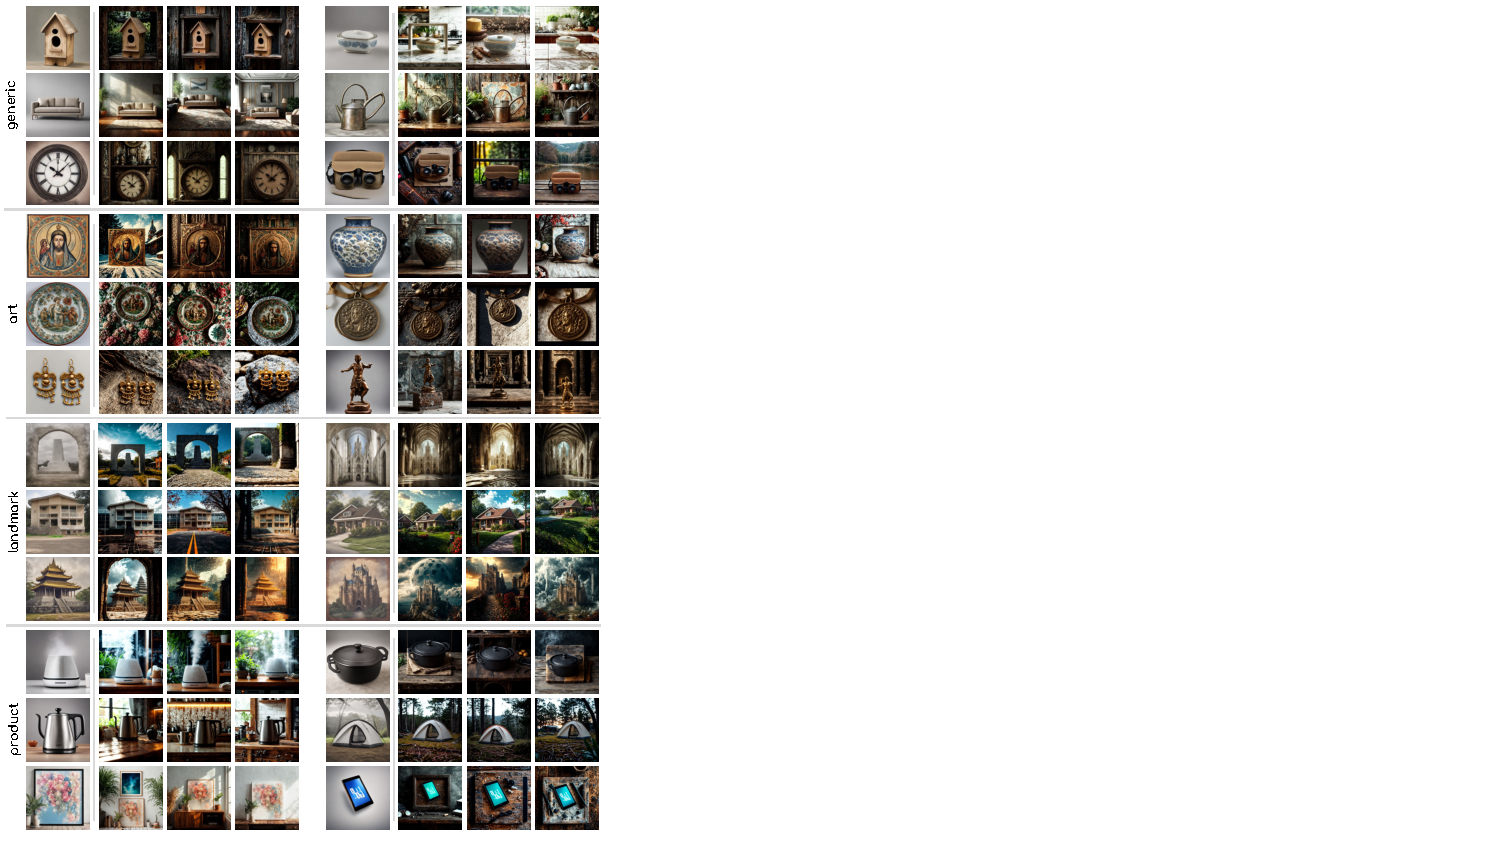
\includegraphics[width=0.91\linewidth]{fig/example.pdf}
\vspace{-9pt}
\caption{Examples of object instances generated by GDM (column 1), and the generated images that leave the object intact and add lighting and background that is well suited to the object (columns 2 $\sim$ 4).
\label{fig:iclight}}
\end{figure*}

\subsection{Representation learning}
%
In total, our generated dataset contains $CKN$ training images, forming $CK$ classes coming from $C$ object categories. 
We construct training batches by sampling $B$ classes and all their corresponding images, resulting in $NB$  images per batch. 
During training, we adopt a query \vs database scheme:
one image from each of the $N$ images per class is randomly chosen as the query, while the remaining $NB-1$ images of the batch form the database, as shown in \cref{fig:batch}.

The similarity between the query and db images is computed in $\hat{\mathbf{y}} \in \mathbb{R}^{NB-1}$, while $\mathbf{y} \in \{0,1\}^{NB-1}$ denotes the labels of all db images with respect to the query, \ie positive or negatives based on their classes. 
We optimize an information retrieval metric as the loss function, in particular an approximation of recall at the top-$k$ ranks, based on $\hat{\mathbf{y}}$, and $\mathbf{y}$.
We train with the average of recall@k loss estimated for different values of $k$.
The approximation of recall is possible by formulating its estimation with the use of step functions, which, during training, are replaced with a sigmoid function.
The technical and implementation details can be found in the original paper~\citep{ptm22}.





\begin{figure}[t]
\begin{center}
\includegraphics[width=0.83\linewidth]{fig/batch.pdf}
\vspace{-10pt}
\caption{Training batch construction for instance-level representation learning. A batch simulates a retrieval task with a query (blue) and database of positive (green) and negative (red) images. Images are considered positive if they belong to the same class, otherwise they are negatives. An image encoder is trained with metric learning on this batch.}
\label{fig:batch}
\end{center}
\end{figure}

\begin{table}[t]
    \centering
    \caption{Statistics of the generated training dataset. \oursgeneric{} and \oursspecific{} comprise only objects from the generic domain and one of the specific domains, respectively.  
    \oursplus{} comprises 50\% of objects from the generic domain ($10$K) and all objects from the three specific domains ($10$K), \ie $20$K objects in total.}
\small
\begin{tabular}{lrrr}
\toprule
\textbf{domain of objects}  & $C$ & $K$ & \textbf{instances} \\ 
\midrule
generic           & $2,000$  & $10$ & $20,000$ \\ 
art        & $200$  & $15$ & $3,000$ \\ 
landmark   & $50$ & $80$  & $4,000$ \\
product    & $200$ & $15$  & $3,000$ \\  
\bottomrule
\end{tabular}

\label{tab:gene_details}
\end{table}



\section{Experiments}

To comprehensively evaluate our approach, we investigate the following Research Questions (RQs):

\textbf{RQ1:} Does MPPReasoner achieve superior performance compared to existing molecular property prediction methods on both ID and OOD datasets?

\textbf{RQ2:} What are the individual contributions of the two-stage training strategy and the RLPGR reward components to the overall performance and reasoning quality?

\textbf{RQ3:} Can our model generate high-quality reasoning paths that provide chemically meaningful insights comparable to expert-level analysis?



\subsection{Experimental Setup}
\label{sec4.1:setup}

\paragraph{Datasets.} 
We evaluate MPPReasoner on 8 diverse molecular property prediction datasets to assess both ID and OOD performance. The datasets are categorized as follows:
\begin{itemize}[leftmargin=*]
\item \textit{ID Datasets:} We utilize four benchmark datasets from MoleculeNet~\citep{moleculenet}, which is widely used to predict whether the given molecule has specific properties: BACE (1,513), BBBP (2,039), SIDER (1,427), HIV (41,127).

\item \textit{OOD Datasets:} We employ four datasets from the Therapeutic Data Commons (TDC)~\citep{tdc1,tdc2} to evaluate cross-task generalization capabilities: Bioavailability (128), CYP2C9\_V (2,418), CYP2D6\_V (2,626), AMES (1,456).
\end{itemize}

The ID/OOD categorization is based on whether the training set includes samples from the corresponding dataset. For training, we randomly sample 4,000 instances from the ID datasets to ensure balanced representation across different molecular properties. Test sets follow standard benchmarking protocols established in prior literature to maintain fair comparison with baseline methods.

\paragraph{Baseline.}
We compare MPPReasoner against two categories of approaches:
\begin{itemize}[leftmargin=*]
\item \textit{Task-specific Specialist Models:} These models are designed for molecular property prediction: Graphormer-p~\citep{graphformer}, Uni-Mol~\citep{unimol}, GIMLET~\citep{gimlet}, MolecularGPT~\citep{moleculargpt}, Mol-LLM~\citep{mol-llm}, InstructMol-GS~\citep{instructmol}, BioT5-Plus~\citep{biot5-plus}, MolXPT~\citep{molxpt}.

\item \textit{LLM-based Generalist Models:} These include reasoning models: o3-mini~\citep{o3mini}, DeepSeek-V3.1~\citep{deepseekr1}, large-scale models: GPT-4o~\citep{gpt4o}, Qwen2.5-VL-72B-Instruct~\citep{qwen25vl}, and baseline models: Qwen2.5-VL-7B-Instruct~\citep{qwen25vl} applied to molecular property prediction.
\end{itemize}

Implementation details and hyper-parameters settings are provided in Appendix~\ref{appc:setting}.




\begin{table}
\setlength{\tabcolsep}{4pt}
\caption{Performance comparison of task-specific specialist models and LLM-based generalist models on ID and OOD benchmarks. Best performance is in \textbf{bold}. }
\label{tab:mol_results}
\centering
\resizebox{\textwidth}{!}{%
\begin{tabular}{lcccc|cccc|cc}
\toprule
\multicolumn{1}{c}{\multirow{2.5}{*}{\textbf{Model}}} 
& \multicolumn{4}{c|}{\textbf{ID Performance}} 
& \multicolumn{4}{c|}{\textbf{OOD Performance}} 
& \multicolumn{2}{c}{\textbf{Average}} \\
\cmidrule(lr){2-5} \cmidrule(lr){6-9} \cmidrule(lr){10-11}
& BACE & BBBP & SIDER & HIV 
& Bioavail. & C2C9\_V & C2D6\_V & AMES
& ID & OOD \\
\midrule
\rowcolor{gray!20}
\multicolumn{11}{c}{\textit{\# Task-specific specialist models}} \\
Graphormer-p   & 0.8575 & 0.7163 & --     & 0.7788 
               & -- & -- & -- & --   
               & 0.7842 & -- \\
Uni-Mol        & 0.8570 & 0.7290 & 0.6590 & \textbf{0.8080} 
               & -- & -- & -- & --   
               & 0.7633 & -- \\
% SCAGE          & 0.8540 & 0.7340 & 0.6600 & -- 
               % & -- & -- & -- & --   
               % & 0.7493 & -- \\
GIMLET         & 0.6957 & 0.5939 & --     & 0.6624 
               & -- & -- & -- & --   
               & 0.6507 & -- \\
MolecularGPT   & 0.7331 & 0.6822 & --     & 0.6382 
               & -- & -- & -- & --   
               & 0.6845 & -- \\
Mol-LLM        & 0.8080 & \textbf{0.8430} & \underline{0.7610} & 0.7650 
               & -- & -- & -- & --   
               & 0.7943 & -- \\
InstructMol-GS & 0.8210 & 0.7240 & --     & 0.6890 
               & -- & -- & -- & --   
               & 0.7447 & -- \\
BioT5-Plus     & 0.8620 & 0.7650 & 0.5201 & 0.7630 
               & 0.5243 & 0.4971 & 0.5321 & 0.4466 
               & 0.7275 & 0.5000 \\
MolXPT         & \underline{0.8840} & \underline{0.8000} & 0.7170 & 0.7810 
               & 0.4749 & 0.5904 & 0.5291 & 0.6073 
               & \underline{0.7955} & 0.5504 \\
\midrule
\rowcolor{gray!20}
\multicolumn{11}{c}{\textit{\# LLM-based generalist models}} \\
o3-mini        & 0.7891 & 0.5972 & 0.5626 & 0.6039 
               & 0.6246 & \underline{0.7729} & \underline{0.7643} & \underline{0.8361} 
               & 0.6382 & \underline{0.7495} \\
DeepSeek-V3.1-Think  & 0.7017 & 0.6048 & 0.5637 & 0.5938 
               & \underline{0.6572} & 0.7633 & 0.7484 & 0.8218 
               & 0.6160 & 0.7477 \\
GPT-4o         & 0.6070 & 0.6731 & 0.6347 & 0.5698 
               & 0.5826 & 0.5508 & 0.5902 & 0.6141 
               & 0.6212 & 0.5844 \\
Qwen2.5-VL-72B-Instruct & 0.7764 & 0.5791 & 0.5880 & 0.7325 
               & 0.6388 & 0.7624 & 0.7222 & 0.8156 
               & 0.6690 & 0.7348 \\ 
Qwen2.5-VL-7B-Instruct  & 0.6910 & 0.6175 & 0.5823 & 0.5125 
               & 0.5232 & 0.7333 & 0.6999 & 0.7667 
               & 0.6008 & 0.6808 \\
\rowcolor{gray!15}
\textbf{MPPReasoner (Ours)} & \textbf{0.9090} & 0.7436 & \textbf{0.8280} & \underline{0.7932} & \textbf{0.6728} & \textbf{0.8480} & \textbf{0.7950} & \textbf{0.8750} & \textbf{0.8190} & \textbf{0.7977} \\
\bottomrule
\end{tabular}}
\end{table}

\subsection{Main Results (RQ1)}

Table~\ref{tab:mol_results} presents the comprehensive performance comparison of MPPReasoner against state-of-the-art baselines across all 8 datasets.
On ID datasets, MPPReasoner demonstrates competitive performance with specialized models while maintaining the advantage of using a smaller 7B parameter architecture. MPPReasoner achieves the best performance on challenging tasks like BACE and SIDER, indicating successful capture of complex molecular property relationships such as enzyme inhibition and side effect prediction. While some specialized models like Mol-LLM excel on specific tasks such as BBBP, these models achieve high ID performance at the expense of cross-task adaptability, completely lacking OOD evaluation capability. This specialization-generalization trade-off limits their practical utility in real-world scenarios requiring diverse molecular property assessment.

The most significant advantage emerges in OOD scenarios, where MPPReasoner substantially outperforms all baseline categories by 6.43\% over the best reasoning model. This consistent superiority across diverse molecular property types highlights how domain-specific chemical reasoning outperforms both general reasoning capabilities and raw parameter scaling approaches. The performance gap becomes even more pronounced when considering that MPPReasoner operates with significantly fewer parameters than competing large-scale models.

The results reveal fundamental differences between model categories and their limitations. Task-specific specialist models excel in familiar scenarios but completely lack cross-task generalization capabilities, while generalist models show consistent cross-task performance but suffer from insufficient domain expertise. MPPReasoner uniquely bridges this gap by embedding domain-specific reasoning rather than relying on general reasoning patterns or parameter scaling alone. The transformative impact becomes evident when comparing MPPReasoner to its base model, showing dramatic improvements of 36.36\% on ID tasks and 17.17\% on OOD tasks. This demonstrates that structured chemical reasoning fundamentally enhances molecular understanding beyond conventional approaches, enabling both specialist-level accuracy and generalist-level adaptability through systematic integration of chemical principles.







\subsection{Ablation Studies (RQ2)}


\begin{table}
\setlength{\tabcolsep}{4pt}
\caption{Ablation study on training stages and RLPGR reward. }
\label{tab:ablation_study}
\centering
\resizebox{\textwidth}{!}{%
\begin{tabular}{lcccc|cccc|cc}
\toprule
\multicolumn{1}{c}{\multirow{2.5}{*}{\textbf{Setting}}} & \multicolumn{4}{c|}{\textbf{ID Performance}} & \multicolumn{4}{c|}{\textbf{OOD Performance}} & \multicolumn{2}{c}{\textbf{Average}} \\
\cmidrule(lr){2-5} \cmidrule(lr){6-9} \cmidrule(lr){10-11}
& BACE & BBBP & SIDER & HIV 
& Bioavail. & C2C9\_V & C2D6\_V & AMES
& ID & OOD \\
\midrule
Base (Qwen2.5-VL-7b-Instruct) & 0.6910 & 0.6175 & 0.5823 & 0.5125 & 0.5232 & 0.7333 & 0.6999 & 0.7667 & 0.6008 & 0.6808 \\
\midrule
SFT Only & 0.8558 & 0.6824 & 0.6752 & 0.7186 & 0.6625 & 0.7799 & 0.7348 & 0.8415 & 0.7330 & 0.7547 \\
RL Only (RLPGR) & 0.8142 & 0.5733 & 0.7428 & 0.5552 & 0.6632 & 0.7491 & 0.6732 & 0.7300 & 0.6714 & 0.7039 \\
\midrule
SFT + $R_{\text{foundation}}$ & 0.8836 & 0.6794 & 0.8089 & 0.7556 & 0.6358 & 0.8364 & 0.7862 & 0.8536 & 0.7819 & 0.7780 \\
SFT + $R_{\text{foundation}}$ + $R_{\text{reasoning}}$ & 0.8877 & 0.7104 & 0.7981 & 0.7560 & \textbf{0.6771} & 0.8140 & 0.7795 & 0.8388 & 0.7881 & 0.7774 \\
\rowcolor{gray!15}
\textbf{MPPReasoner (Ours)} & \textbf{0.9090} & \textbf{0.7459} & \textbf{0.8280} & \textbf{0.7932} & 0.6728 & \textbf{0.8480} & \textbf{0.7950} & \textbf{0.8750} & \textbf{0.8190} & \textbf{0.7977} \\
\bottomrule
\end{tabular}}
\end{table}


To understand the individual contributions of our two-stage training strategy and the hierarchical reward components in RLPGR, we conduct comprehensive ablation studies. Table~\ref{tab:ablation_study} presents the systematic analysis of each component's impact on both ID and OOD performance.
The results demonstrate that both SFT and RL stages contribute significantly to overall performance, with distinct advantages for different aspects. SFT alone provides substantial improvements over the base model, achieving 22.01\% and 10.85\% gains on ID and OOD tasks respectively, indicating that SFT with high-quality reasoning trajectories successfully instills foundational chemical reasoning capabilities. RL alone also shows meaningful improvements of 11.74\% and 3.39\%, demonstrating that principle-guided rewards can enhance reasoning quality independently. However, the combination of SFT + RL yields the strongest performance with 36.36\% and 17.17\% improvements, revealing important synergistic effects between two training stages that exceed their individual contributions.

The progressive addition of RLPGR reward components shows clear incremental benefits, validating our hierarchical design. Foundation rewards provide substantial improvements of 6.67\% on ID and 3.09\% on OOD over SFT alone, establishing enhanced task completion capabilities beyond basic instruction following. The Reasoning layer contributes additional 0.84\% ID gains while maintaining similar OOD performance, indicating that logical consistency and comparative analysis refine reasoning quality without compromising generalization. Most importantly, the Chemistry layer delivers the largest incremental improvements of 3.92\% on ID and 2.61\% on OOD, confirming that domain-specific chemical principle verification is crucial for molecular property prediction tasks.




\subsection{Reasoning Quality Evaluation (RQ3)}
\label{sec4.4:quality}
\begin{figure}
    \centering
    \begin{subfigure}[b]{0.49\textwidth}
        \centering
        \includegraphics[width=\textwidth]{figs/score_dist.png}
        % \caption{}
        \caption{Human-AI evaluation consistency}
        \label{fig:score_distribution}
    \end{subfigure}
    \hfill
    \begin{subfigure}[b]{0.49\textwidth}
        \centering
        \includegraphics[width=\textwidth]{figs/score.pdf}
        % \caption{}
        \caption{Model reasoning quality scores}
        \label{fig:model_performance}
    \end{subfigure}
    \vspace{-1em}
    \caption{Reasoning quality evaluation results. (a) Strong consistency between automated and human assessments with $\rho$ = 0.82. (b) MPPReasoner achieves the highest reasoning quality score.}
    \label{fig:reasoning_evaluation}
\end{figure}

To assess whether MPPReasoner generates high-quality reasoning paths that provide chemically meaningful insights, we conduct systematic evaluation using automated assessment validated against human expert judgment. We employ a LLM-as-a-Judge~\citep{llmasjudge} framework using GPT-4o to evaluate three dimensions~\citep{sophiavlr1}: \textbf{logical soundness, accuracy \& insight, and conciseness}, each scored on a 0-10 scale with detailed rubrics. To establish reliability, we validate GPT-4o scores against human expert assessments on 60 reasoning samples from three baseline models. Figure~\ref{fig:reasoning_evaluation}(a) shows remarkable consistency between automated and human evaluations, with similar distributions and central tendencies with spearman correlation coefficient reaches $\rho$ = 0.82.

Figure~\ref{fig:reasoning_evaluation}(b) presents the comparative reasoning quality assessment across different model categories, showing average scores across the three evaluation dimensions. MPPReasoner achieves the highest score of 7.730, substantially outperforming advanced reasoning models including DeepSeek-V3.1-Think at 6.723 and o3-mini at 6.235, as well as large-scale models like Qwen2.5-VL-72B at 6.458 and GPT-4o at 6.089. Despite using a smaller 7B architecture, MPPReasoner demonstrates 15.0\% improvement over the best baseline, highlighting how domain-specific chemical reasoning surpasses both general reasoning capabilities and parameter scaling approaches. The superior reasoning quality translates to practical benefits: MPPReasoner consistently identifies relevant functional groups, applies appropriate chemical principles, and provides mechanistic explanations that enable chemists to understand both what properties a molecule has and why these properties emerge from specific structural features. Detailed dimensional scores are provided in Appendix~\ref{appb:quality}.

\section{Limitations}
\label{sec:limitations}

While our approach effectively generates precise and detailed expressions, some limitations remain. First, the adopted parametric representation lacks semantic interpretability. As a result, expression manipulation typically relies on extracting parameters from reference images, which may be limiting for certain applications. Second, the accuracy of expression reproduction is inherently dependent on the quality of the 3D reconstruction method used to extract blendshape parameters~\cite{smirk_2024_CVPR}, which although state-of-the-art might still be imperfect and introduce occasional errors. Finally, expression editing with the \textbf{Reference Adapter} can sometimes be inconsistent. As shown in \cref{fig:failure_cases} (top), there are instances where the base model accurately transfers the target expression, but the reference-driven variant fails to do so. This is due to the \textbf{Reference Adapter} often tending to ``copy-paste'' the reference image, despite our use of cross-paired video data for training. This behavior can be mitigated at test time by adjusting the scaling factor $\lambda$ of the LoRA layers, which modulates the influence of the reference image. As shown in \cref{fig:failure_cases} (bottom), reducing $\lambda$ improves expression fidelity at the cost of slight deviations in background or pose from the reference image.
\\
\noindent \textbf{Note on social impact.} We acknowledge the ethical implications of our work, as technologies for controllable face generation may be misused to produce deceptive or unoriginal facial imagery, particularly when capable of altering expressions. While our goal is to advance research in positive domains such as accessibility and creative storytelling, we recognize these risks and emphasize the importance of ethical standards and investment in countermeasures like synthetic content detection.

\begin{figure}[h]
\centering
\includegraphics[width=1.0\linewidth]{figures/failure_cases_compressed.pdf}
\caption{\textbf{Top:} Example of failure case where the base model successfully reproduces the target expression, but the reference-driven variant struggles due to over-reliance on the source image. \textbf{Bottom:} Reducing the LoRA scaling factor $\lambda$ of the Reference Adapter alleviates this by trading off pose and background consistency for improved expression fidelity.}
\label{fig:failure_cases}
\end{figure}


\vspace{-0.7em}
\section{Conclusion}
\vspace{-0.7em}



In this paper, we introduce \textbf{\method{}}, a safety-aligned reinforcement learning framework that embeds safety as an active driver of multimodal reasoning. By integrating the curated QI-Safe-10K dataset, safety-aware rollouts with reflection and correction, and structured reward modeling, \method{} shifts safety from a passive safeguard to a core component of inference. Extensive evaluations show that it achieves SOTA safety and competitive helpfulness, surpasses same-scale and larger open-source models, and performs on par with leading proprietary systems. Robustness and ablation studies confirm that the improvements stem from injecting safety-awareness into the reasoning process. Together, these results establish \method{} as a reliable paradigm for multimodal safety alignment and a foundation for building future safe and interpretable AI systems.





{
    \small
    \bibliographystyle{ieeenat_fullname}
    \bibliography{main}
}

\section*{Appendix Overview}

The appendix includes extra experimental results, corresponding analyses, and further discussions of IF-V2V. The appendix is organized as follows:
\begin{itemize}
    \item \sref{sec:diagnostic_lambda} analyzes the effect of the rectification scale in \sref{sec:vfr-sd}.
    \item \sref{sec:abl_smpi} further ablates the components of SMPI.
    \item \sref{sec:comp_solver} provides comparisons on adopting different ODE solvers.
    \item \sref{sec:ext_flow} demonstrates quantitative and qualitative results of extending IF-V2V to other flow-based I2V models for editing.
    \item \sref{sec:t2v_edit} presents qualitative results of extending IF-V2V for text-guided video editing.
    \item \sref{sec:image_edit} adapts an inversion-free image editing method FlowEdit~\citep{kulikov2024floweditinversionfreetextbasedediting} to the video domain for quantitative comparison.
    \item \sref{sec:vis_extra} shows more qualitative results of IF-V2V.
    \item \sref{sec:discussions} further discusses the theoretical justifications, hyperparameter selection criteria, limitations, and societal impacts of IF-V2V.
\end{itemize}

\section{Effect of the Rectification Scale}
\label{sec:diagnostic_lambda}

\begin{figure}[ht]
  \centering
  \includegraphics[width=\linewidth]{figs/vis_lambda.pdf}
  \caption{Illustration of the effect of the rectification scale $\lambda$ (\sref{sec:diagnostic_lambda}). The source video shows a boy in a \textbf{white} T-shirt cycling along the road, and the edited first frame changes the boy's T-shirt to \textbf{red}. The value of $\lambda$ can be tuned in an appropriate range to control the strength of the source video prior. A small $\lambda$ ($\leq 0.50$) brings a weak prior from the source video, resulting in inconsistency with the source video that the boy cycles along a road with an endless wall. When $\lambda$ is too large ($\geq 1.25$), artifacts like blurs and oversaturation also emerge. Please zoom in for details.}
  \label{fig:lambda}
\end{figure}

The rectification scale $\lambda$ in \sref{sec:vfr-sd} determines the strength that VFR-SD incorporates the source video's deviation from expectation during the target ODE solving process. To provide an intuitive understanding of the impact of $\lambda$ on the edited video, we present a visualization of using different values of $\lambda$ to edit a video sample in \cref{fig:lambda}. The video originally captures a boy in a white T-shirt cycling along the road, and the edited frame turns the boy's T-shirt red. When $\lambda$ is small ($\leq 0.5$), the deviation from the source video is relatively weak, and the denoising process resembles the straightforward I2V process. In this case, the sample deviation is inadequate to direct the denoising process, resulting in the boy cycling along the road with an \textit{endless} wall. In contrast, an overly large $\lambda$ value ($\geq 1.25$) also induces artifacts like blurs and oversaturation because the rectification term pushes the generated sample too far from the original distribution.

\section{Extra Ablations on SMPI}
\label{sec:abl_smpi}

We conduct extra ablations to provide a better understanding of SMPI. The results are displayed in \cref{tab:abl_smpi}, where \textit{w/o} MPI stands for without motion-preserving initialization. Comparing \#1 and \#2, we can observe that structure-preserving initialization better maintains the consistency with original videos (OVC). From \#2 and \#3, it can be concluded that motion-preserving initialization further enhances temporal consistency.

\begin{table}[ht]
  \caption{Quantitative ablations on SMPI (\sref{sec:abl_smpi}). Results in \textbf{bold} are the best.
  }
  \label{tab:abl_smpi}
  \centering
  \begin{tabular}{l|ccccc|c}
    \toprule
    Setting & AS & TC & EFC & OVC & AEC & Time \\
    \midrule
    \textit{w/o} SMPI & 4.78 & 98.19 & 92.67 & 75.45 & 84.06 & 622.38 \\
    \textit{w/o} MPI & 4.81 & 98.06 & 92.51 & 76.30 & 84.41 & \textbf{615.17} \\
    IF-V2V & \textbf{4.88} & \textbf{98.71} & \textbf{92.79} & \textbf{76.44} & \textbf{84.62} & 616.60 \\
    \bottomrule
  \end{tabular}
\end{table}

\section{Comparisons on ODE Solvers}
\label{sec:comp_solver}

To validate IF-V2V's compatibility with different ODE solvers, we evaluate IF-V2V's performance with Euler Discrete Scheduler~\citep{sd3} and UniPC Scheduler~\citep{unipc}. Quantitative results are displayed in \cref{tab:comp_solver} with the same settings as \sref{sec:diagnostic}. We also present qualitative results in \cref{fig:vis_solver}. From the above results, we can conclude that IF-V2V also achieves satisfactory performance with UniPC Scheduler~\citep{unipc}, demonstrating the universality of our method.

\begin{table}
  \caption{Comparisons on adopting different ODE solvers in IF-V2V (\sref{sec:comp_solver}).
  % Results in \textbf{bold} are the best.
  }
  \label{tab:comp_solver}
  \centering
  \begin{tabular}{l|ccccc}
    \toprule
    Setting & AS & TC & EFC & OVC & AEC \\
    \midrule
    UniPC~\citep{unipc} & 4.86 & 98.70 & 92.01 & 76.48 & 84.25  \\
    Euler~\citep{sd3} & 4.88 & 98.71 & 92.79 & 76.44 & 84.62 \\
    \bottomrule
  \end{tabular}
\end{table}

\begin{figure}[ht]
  \centering
  \includegraphics[width=\linewidth]{figs_supp/vis_solver.pdf}
  \caption{Visualizations of using different ODE solvers in IF-V2V (\sref{sec:comp_solver}). The edited first frame is in the bottom-right corner of the edited video. IF-V2V is compatible with multiple ODE solvers to produce high-quality editing results.}
  \label{fig:vis_solver}
\end{figure}

\section{Extension to Other Flow-based I2V Models}
\label{sec:ext_flow}

\begin{table}
  \caption{Comparisons on using different I2V models in IF-V2V (\sref{sec:ext_flow}).
  % Results in \textbf{bold} are the best.
  }
  \label{tab:comp_flow}
  \centering
  \begin{tabular}{l|ccccc}
    \toprule
    Setting & AS & TC & EFC & OVC & AEC \\
    \midrule
    % \makecell[l]{HunyuanVideo\\\citep{hunyuanvideo}} & 4.75 & 98.60 & 92.92 & 75.36 & 84.14  \\
    HunyuanVideo~\citep{hunyuanvideo} & 4.75 & 98.60 & 92.92 & 75.36 & 84.14  \\
    Wan2.1~\citep{wan} & 4.88 & 98.71 & 92.79 & 76.44 & 84.62 \\
    \bottomrule
  \end{tabular}
\end{table}

\begin{figure}
  \centering
  \includegraphics[width=\linewidth]{figs_supp/vis_hunyuan.pdf}
  \caption{Editing samples of using different flow-based I2V models in IF-V2V (\sref{sec:ext_flow}). The edited first frame is in the bottom-right corner of the source video. IF-V2V can be applied to various flow-based I2V models for high-quality video editing.}
  \label{fig:vis_hunyuan}
\end{figure}

To further demonstrate the universality of IF-V2V, we select HunyuanVideo~\citep{hunyuanvideo} as another base I2V model to apply our method. We present the quantitative results in \cref{tab:comp_flow}, from which we can find that HunyuanVideo~\citep{hunyuanvideo} also achieves a satisfying result that surpasses prior arts. \cref{fig:vis_hunyuan} shows the visualization of some editing cases, in which we can observe that both HunyuanVideo~\citep{hunyuanvideo} and Wan2.1~\citep{wan} achieve excellent consistency with both the edited frame and the original video with the help of IF-V2V.

\section{Extension to Text-guided Editing}
\label{sec:t2v_edit}

\begin{figure}
  \centering
  \includegraphics[width=\linewidth]{figs_supp/vis_t2v.pdf}
  \caption{Text-guided editing results of IF-V2V (\sref{sec:t2v_edit}). We provide the simplified editing caption under each sample. Compared to \textit{I2V + Init}, our method preserves the details more faithfully, like shells and splashes in (a), and aligns better with the editing instruction, such as the guitar in (b).}
  \label{fig:vis_t2v}
\end{figure}

IF-V2V can also be used for text-guided video editing by removing the condition embedding in Structure-Preserving Initialization. We present some qualitative results using Wan2.1~\citep{wan} as the text-to-video model in \cref{fig:vis_t2v}, in which we can observe that IF-V2V also achieves excellent consistency and editing quality. In \cref{fig:vis_t2v} (a), IF-V2V keeps the details more faithfully, such as shells on the beach and splashes in the sea, compared to directly blending Gaussian noise and source video latents as the initial condition for the I2V model (I2V + Init). In \cref{fig:vis_t2v} (b), IF-V2V also aligns better with the editing prompt that alters the electric guitar into a normal one.

\section{Quantitative Comparisons with FlowEdit}
\label{sec:image_edit}

To demonstrate the superiority of IF-V2V over directly adopting image-based inversion-free editing methods for videos, we adapt FlowEdit~\citep{kulikov2024floweditinversionfreetextbasedediting}, a flow-based inversion-free image editing method, for video editing on Wan2.1~\citep{wan}. The performance is displayed in \cref{tab:comp_flowedit}, from which we can observe that both its editing quality and inference speed remain inferior to IF-V2V. This further validates the effectiveness of our new perspective on the ODE solving process, video-specific designs, and flexible caching strategy.

\begin{table}
  \caption{Quantitative comparisons with FlowEdit (\sref{sec:image_edit}). Results in \textbf{bold} are the best.}
  \label{tab:comp_flowedit}
  \centering
  \begin{tabular}{l|ccc|c}
    \toprule
    Setting & AS & TC & EFC & Time \\
    \midrule
    FlowEdit~\citep{kulikov2024floweditinversionfreetextbasedediting} & 4.76 & 98.01 & 92.32 & 802.42 \\
    IF-V2V (Ours) & \textbf{4.88} & \textbf{98.71} & \textbf{92.79} & \textbf{616.60}\\
    \bottomrule
  \end{tabular}
\end{table}

\section{More Visualizations}
\label{sec:vis_extra}

We illustrate more editing results of IF-V2V in \cref{fig:vis_extra}, which include object addition (a), object removal (b), and attribute modification (c). As observed, IF-V2V consistently achieves satisfactory performance on various video editing tasks. Please refer to the supplementary video for dynamic versions of editing samples.

\begin{figure}
  \centering
  \includegraphics[width=\linewidth]{figs/vis_extra.pdf}
  \caption{More visualizations of editing results of IF-V2V (\sref{sec:vis_extra}). The edited first frame is in the bottom-right corner of the source video. The cases include object addition (a), object removal (b), and attribute modification (c). Our method propagates the edited frame to the whole video with excellent quality and consistency.
  }
  \label{fig:vis_extra}
\end{figure}

\section{More Discussions}
\label{sec:discussions}

\subsection{Theoretical Justifications}
\label{sec:theoretical}
IF-V2V shares a similar theoretical basis as inversion-based editing methods: Optimal Transport (OT) mapping between the source and target distribution. The theoretical difference is that inversion-based methods conduct a mapping on the marginal distribution $p(z_0|z_{t_{max}})$, while IF-V2V performs mappings on transition distributions $p(z_{t-\Delta t} |z_t)$. When \(\Delta t\) is small enough, both the source and target transition distributions can be viewed as Gaussians with the same variance~\citep{ddpm, gmflow}. In this case, IF-V2V with $\lambda=1$ performs the exact OT mapping on the transitions.

\subsection{Hyperparameter Selection}
\label{sec:hyperparam}

The editing results suffer from over-saturation and distortion when the rectification scale $\lambda$ in \sref{sec:vfr-sd} is overly large. When the edited frame is not aligned with the original frame, the rectification sometimes causes unintended drifts due to the conflict. The scale of structure-preserving initialization $\beta$ in \sref{sec:spi} should be small enough when the edited region is large. Otherwise, IF-V2V mostly preserves the original video. An overly large flow-guided initialization factor $\alpha$ in \sref{sec:mpi} breaks the temporal Gaussianity of the noise and fails the generation.

It has been discovered that initial steps are more crucial for editing, and the vector difference in these steps is also larger. The caching threshold $\delta$ in \sref{sec:dcache} is selected around the vector difference in early steps to avoid caching these steps. Caching in later steps reduces computational cost with less impact on editing quality.

\subsection{Limitations}
\label{sec:limitations}

The editing capability of our method is inherently bounded by the selected image editing model and the I2V model. Failure in either stage will result in unsatisfactory results. Moreover, since existing I2V models only predict the expectation of the distribution without covariance information, IF-V2V cannot exploit the covariance to achieve more precise mapping from the source sample to the target sample in a training-free way. 

\subsubsection{Image Editing Methods}
\label{sec:limitations_imageedit}

IF-V2V's editing results rely on the first frame edited by image editing methods. However, current state-of-the-art methods~\citep{gpt4oimg, stepedit} still suffer from inconsistencies and trial-and-error. For instance, the image edited by GPT-4o~\citep{gpt4oimg} often misaligns with the original image, especially when changing the original image into a significantly different style (\eg, Ghibli cartoonish style). Such misalignment may cause undesired alterations in the edited videos. In addition, Step1X-Edit~\citep{stepedit} sometimes needs several tries to achieve a satisfactory editing result. We expect that the future advancements of image editing methods will ease the process of obtaining a satisfactory first frame and further boost the performance of IF-V2V.

\subsubsection{I2V Models}
\label{sec:limitations_i2v}

\begin{figure}
  \centering
  \includegraphics[width=\linewidth]{figs_supp/vis_failure.pdf}
  \caption{Failure cases of IF-V2V (\sref{sec:limitations_i2v}). The edited first frame is in the bottom-right corner of the source video. IF-V2V struggles to handle editing samples with overly complex (a) or fast (b) motions due to the limited capability of I2V models.}
  \label{fig:failure}
\end{figure}

IF-V2V fails to produce satisfactory results when motion in the source video is overly complex or fast. As \cref{fig:failure} (a) displays, when there are complicated motions in the source video like simultaneous multiple subject movement with changing occlusions, IF-V2V cannot genuinely reproduce such motion in the edited video. In \cref{fig:failure} (b), IF-V2V generates unsatisfactory results when dealing with breakdance, which contains rapid human body movements. These phenomena stem from state-of-the-art I2V models' limited ability to generate rapid or sophisticated motions. This problem may be resolved by more powerful I2V models in the future which are capable of handling such complex motions.

Furthermore, mainstream flow-based I2V models~\citep{wan, easyanimate, hunyuanvideo, cogvideox, opensora2, vchitect2} only predict the \textit{expectation} of the target distribution without further information like covariance, making it hard to conduct more fine-grained operations to map the source sample to the target distribution in a training-free way. This may limit the method's ability to maintain the consistency of fine-grained details in edited videos.

\subsection{Societal Impacts}
\label{sec:impacts}

IF-V2V can achieve high-quality video editing by combining off-the-shelf image editing and I2V methods without training, enabling practitioners to flexibly leverage the most up-to-date models to implement their creativity. For individual creators, the lightweight nature of our method enables them to introduce AI-assisted video content creation into their workflow, democratizing the application of advanced AIGC tools. This shift can also expand storytelling beyond traditional media institutions to include diverse voices and perspectives. For commercial teams, our method provides them with a new chance to flexibly combine their internal results or models with the progress of the open-source community, boosting the quality of the produced videos with minor extra cost.

On the other hand, with IF-V2V's powerful capability of manipulating objects and attributes in the video, it can produce fabricated videos that appear highly realistic, posing significant challenges for verifying the authenticity of visual media. Such content can distort public perception and raise privacy concerns when fake contents featuring an individual are generated in an unauthorized way.


\end{document}
